%% notes-tex/multimodal/043-training-design/sections/2-flow.tex
%% SOURCE: the diagram's numbers and their files are listed in its Dendron note,
%% notes/experiments.043-expression-proteome-morphology.mermaid.training-design.md

\section{Data and model flow\secstatus{todo}}
\label{sec:flow}

Figure~\ref{fig:flow} follows a record from the raw store to the number the decision rule
reads. The store and its datasets are described in the 043 datasets primer
(\file{notes-tex/multimodal/043-datasets-primer/}, Secs.\ 1 to 4 and 6); what follows starts
where the primer stops, at the representation the trainer consumes. Two facts set the
shape of the pipeline. First, the representation holds keys, not vectors: each gene slot
of a reference context carries one key per frozen block, or a typed gap, and the trainer
reads the vectors of exactly the keys its records use, failing on a missing one.
Second, the reference context is part of the input: a deletion, segregant or promoter
record is read on S288C, an isolate on its own alleles (route A), so a batch carries
between one and $B$ distinct contexts, and the trunk runs once per distinct context.

%% SOURCE: notes/experiments.043-expression-proteome-morphology.mermaid.training-design.md, rendered by
%% notes/assets/publish/scripts/mermaid_pdf.sh, copied and scaled to 180 mm by `make diagrams`
\begin{figure}[htbp]\centering
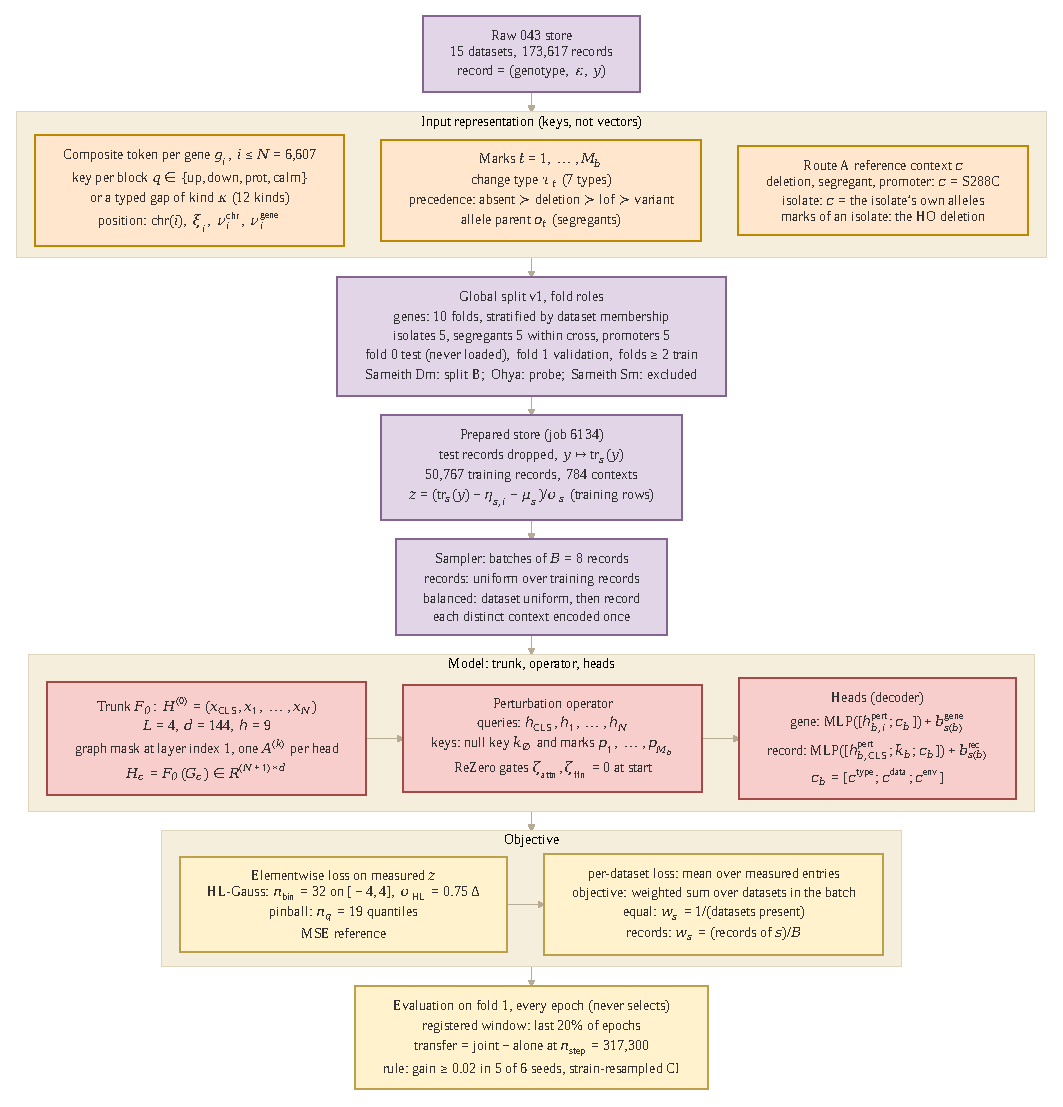
\includegraphics[width=\textwidth]{figures/mermaid-training-design.pdf}\par\vspace{2pt}
\caption[]{\textbf{The 043 training pipeline, from the raw store to the
registered-window read.} Purple, data: the store, the fold roles of the global split, the
prepared store (job 6134; test records dropped before any label is loaded) and the batch.
Orange, input side: the composite token per gene with its position features, the marks
with their change types and allele parents, and the route-A reference context. Red,
model: trunk, perturbation operator and heads. Yellow, objective and evaluation. The 784
contexts of the prepared store are S288C and the 783 isolates outside fold 0. In the
rendered math, vectors written bold in the text ($\mathbf{c}_b$, $\mathbf{p}_t$,
$\bar{\mathbf{k}}_b$) appear in the regular face. Rendered 212 mm wide and placed at
180 mm, a scale of 0.85.}
\label{fig:flow}
\end{figure}
%% Generated by notes/assets/publish/scripts/mermaid_pdf.sh from
%% notes/experiments.043-expression-proteome-morphology.mermaid.training-design.md

\notesec{Stages}
The global split assigns every record one role before anything trains
(Sec.~\ref{sec:split}). The prepare stage (\file{train_043.py} \texttt{-{}-stage prepare}, job 6134)
reads every record of the arm's datasets with its route-A representation, drops the test
records, applies the per-dataset transform $\operatorname{tr}_s$ and writes keys, marks,
contexts, targets and the nine gene--gene edge lists into one store. Training fits the
standardization on the training rows, builds the model, and logs the training objective
every 50 steps and the validation pass every evaluation epoch. Nothing downstream of the
prepared store reads fold 0.
